
\newcommand{\pms}{OPUS~}
\newcommand{\pmslong}{Online Placement University System}
\newcommand{\pmsurl}{http://opus.ulster.ac.uk}


\documentclass{article}
\usepackage[pdftex]{graphicx}
\usepackage{hyperref}
\usepackage{url}
\usepackage{amsfonts}
\usepackage{fancyheadings}
\usepackage{lastpage}
\DeclareGraphicsExtensions{.pdf,.../Figures/png,.mps}

\usepackage{url}
\usepackage{hyperref}

\pagestyle{fancy}
\lhead{\pmslong}
\chead{}
\rhead{Company Hireing Guide}
\lfoot{\url{\pmsurl}}
\cfoot{\thepage / \pageref{LastPage}}
\rfoot{}
\setlength{\headrulewidth}{0.4pt}
\setlength{\footrulewidth}{0.4pt}

\author{Dr C R Turner}

\title{\pmslong \\ Company Guide - Hiring Students}


\begin{document}

\maketitle
\newpage
\section{Introduction}

This guide is aimed at those who are interesting in hiring a placement student from the
University of Ulster. The university has a web based system, the \pmslong (\pms),
which is used to help you advertise for the best student for your vacancy. At the time of
writing the system is in wide use in the Faculty of Engineering and is rolling out further.
You may not be able to use the system if the school or faculty you normally do business with
does not yet use it, or if your placement is not chosen by competitive selection.

The system also supports students in placement, and there is a separate document
% @todo come back to this
which looks at how the system can help you manage a student who is placed with you.

\section{Getting Started}.

If you have not already got an account on the \pms then please speak to your normal contact
for placement within the University, or email
% @todo add an email address here
to have an account made for you.

When you have your login details, you can login at \url{\pmsurl}.

When you login, you will see something like the following
\begin{figure}[htb]
\begin{center}
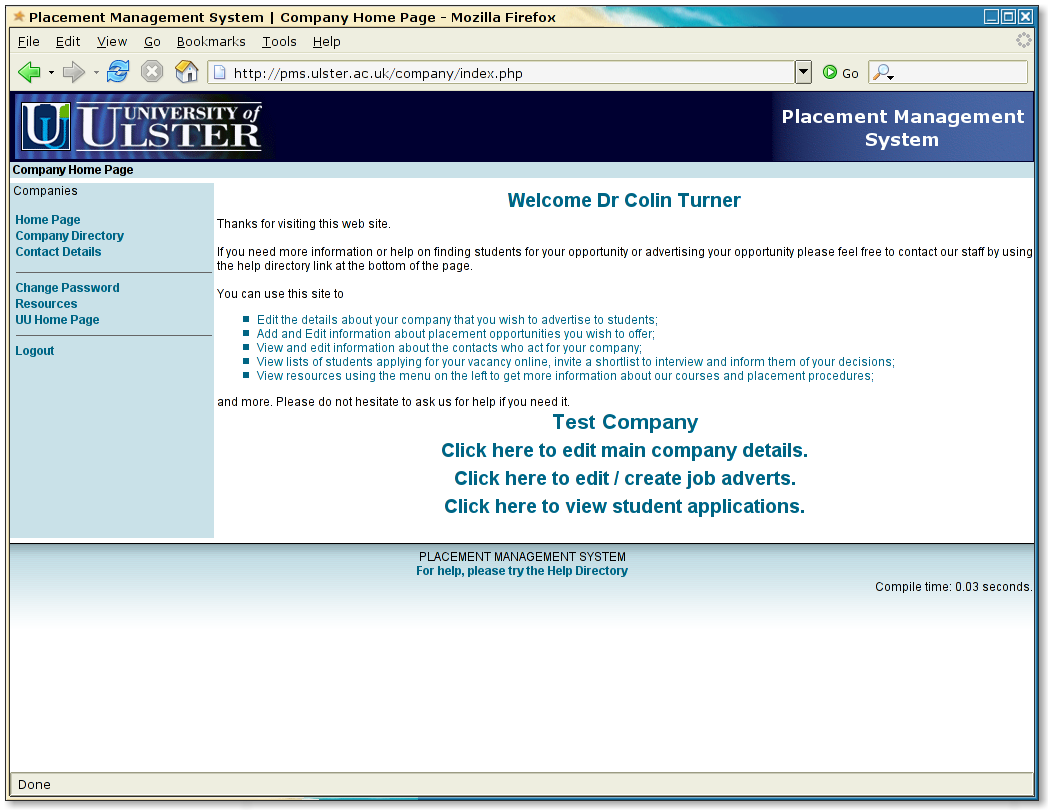
\includegraphics[scale=0.25]{png/company_hr1.png}
\end{center}
\end{figure}
On the left hand side you will see a menu. That menu will remain available to you
at all times. At any time clicking on ``Home Page'' will return you here. The other menu
items in turn are

\begin{description}
\item[Company Directory] allows you to search through other companies on the system;
\item[Contact Details] allows you to check and edit your own contact details;
\item[Change Password] allows you to alter the preconfigured password;
\item[Resources] provides a large collection of documents to guide you;
\item[UU Home Page] takes you the main university home page;
\item[Logout] logs you out from the system.
\end{description}

At any time, clicking on the link for the ``Help Directory'' will
provide you with details on the staff who are most likely to be
able to help with your enquiries.


\subsection{Checking the Company Details}

Possibly the first thing you may want to do (especially if this is your first visit to
the system), is to check over the company information. At the bottom of the main screen
it says ``Click here to edit main company details''.

\begin{figure}[htb]
\begin{center}
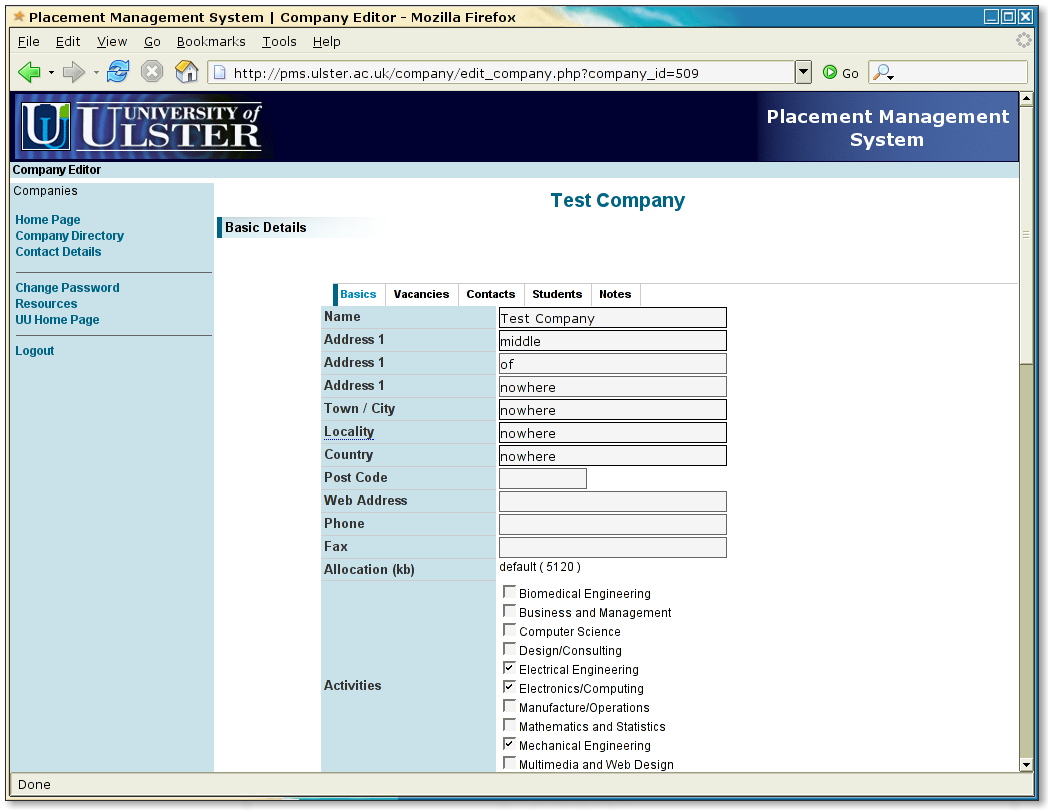
\includegraphics[scale=0.25]{png/company_hr2.png}
\end{center}
\end{figure}


Clicking on this will take you to a page that allows you to edit much about your company,
including the basic contact details. You will also notice that above this area there is
a collection of other headers such as ``Vacancies'' etc., these provide another means of
navigating your record.

Be sure to check your company information is correct. Please note that students are not
shown phone numbers so that they will not bother you directly. You can insert these in the
company brief if you want students to have this information. In the ``Locality'' field please
enter the geographical region of your company. Within the UK and Ireland this could be a
county, or within the areas of larger cities such as Belfast or Dublin please enter the
city name.

Towards the bottom of the form there are other areas to explore.

\begin{figure}[htb]
\begin{center}
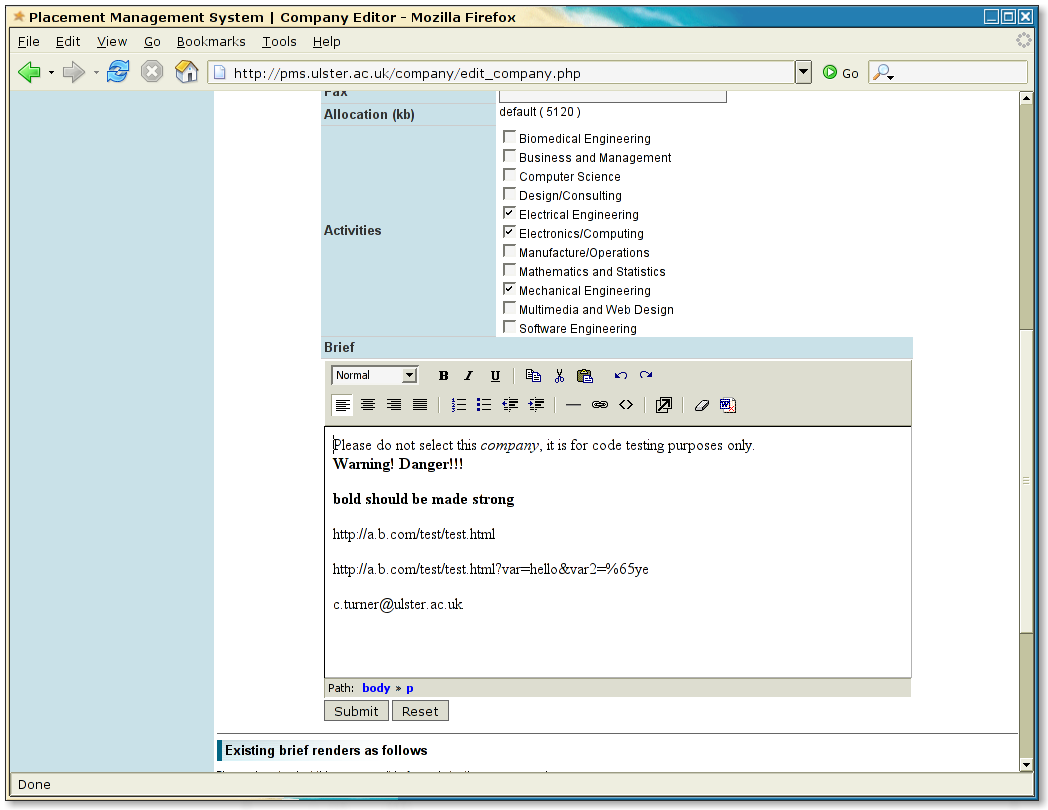
\includegraphics[scale=0.25]{png/company_hr3.png}
\end{center}
\end{figure}


File allocation is an amount of memory for you to use to upload resources, these are PDF
documents to further describe your company, or application forms or similar. If you require more, please contact an administrator
from your help directory.

Activities allows you to indicate in which areas your company does business. Note that you will have a separate opportunity to list activities for your vacancies, so this is a chance to describe all the areas your company is active in.

Finally we have the brief. This is an area in which you can
describe your company to the students. An editor is available in
all modern browsers to allow you to edit this content.

Make your edits as you wish and then save them.

\section{Advertising your vacancy}

Next you will wish to move on to posting your advert for your
vacancy or perhaps you wish to advertise several opportunities.

Clicking on the ``vacancies'' tab of the display will take you
where you need to go
\begin{figure}[htb]
\begin{center}
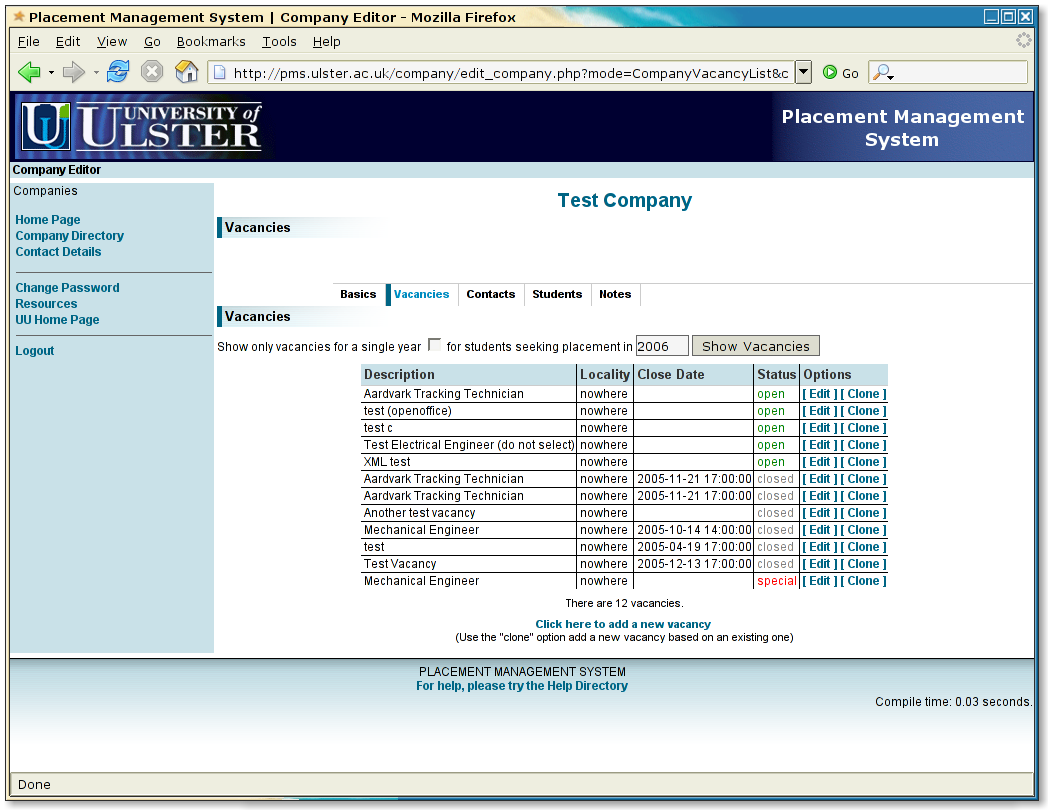
\includegraphics[scale=0.25]{png/company_hr4.png}
\end{center}
\end{figure}


The page will list the vacancies you already have on the system
(if any). You can ``edit'' an existing vacancy, by clicking on
``edit'' to the right. Using the ``clone'' option starts a new
vacancy, but using the existing one as a template to start with.

Many times you will want to create a new vacancy from scratch,
and for this click on the link at the bottom of the page.

Adding a vacancy is similar to editing your company brief.
Here are some points to help your

\begin{description}
\item[Description] is a summary of your proposed vacancy. Where
possible be as descriptive as possible, and try to avoid
``placement student''.
\item[Job Start Date] is essential to the system. It will use it to
decide which students should be shown your vacancy. If you are 
unsure use a provisional date in the area you are planning, you
can always change it later.
\item[Application Close Date] is not compulsory, but if you set
one the system will automatically close your vacancy after this
date and email you a notification.
\item[Application Status] can be one of open, closed and special.
Vacancies that are ``open'' can be applied for on-line and you
will be able to use the full facilities of the system. The
status ``special'' indicates vacancies where the application
cannot be made on our website because of some restriction you
may have. Finally ``closed'' indicated applications are no
longer possible. Vacancies will close automatically after the
closing date passes (if you have declared one).
\end{description}

\section{Checking and selecting students}

By clicking on the ``Students'' tab you will be able to see
the applications made to your vacancies. All vacancies will be
listed for a specific year.
\begin{figure}[htb]
\begin{center}
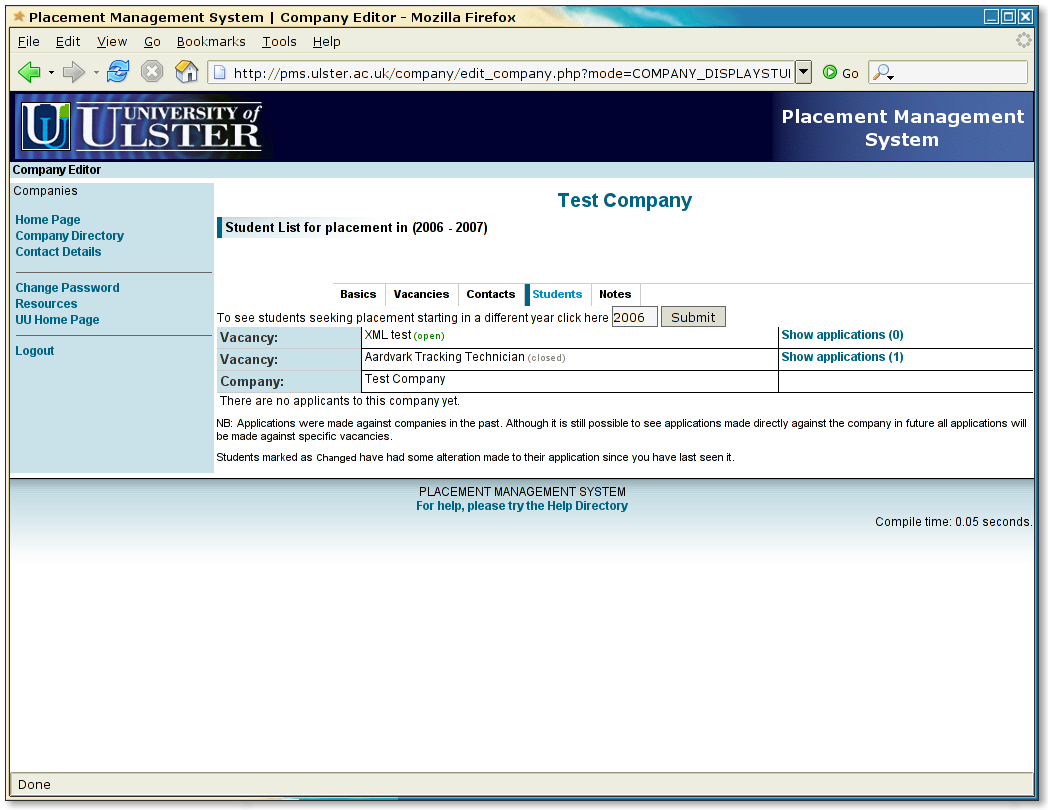
\includegraphics[scale=0.25]{png/company_hr5.png}
\end{center}
\end{figure}

Click on ``Show applications'' for a specific vacancy to see
what students have applied.

Student lists are triaged as follows
\begin{itemize}
\item students you have selected for this vacancy;
\item students who are still available;
\item students who applied but are no longer available (e.g. they are placed elsewhere).
\end{itemize}

For each student you will see
\begin{itemize}
\item their name; clicking on this produces their CV;
\item their course of study;
\item whether their application has changed since you have last seen it;
\item their application date, and any date of modification;
\item a link for who can help with \emph{this} student;
\item a form to allow you to change their status;
\item and a link to request a CV to be emailled to you.
\end{itemize}

You can then call students to email, or use the form to do this
for you.

\section{What Next?}

When you have accepted students you can use the form in their
entry to inform them of this, and we would also ask you to
inform your contact within the university. The university will
then record the student as being placed with your company.

\end{document}